\section{The \emph{Compact Muon Solenoid} experiment}
%%%%%%%%%%%%%%%%%%%%%%%%%%%%%%%%%%%%%%%%%
\label{sec:CMS}

The CMS apparatus is a general purpose detector situated in one of the four LHC interaction points\footnote{The CMS detector is placed in a cavern 100\,m underground in the area called Point 5, near the village of Cessy, in France.}. The detector is designed to investigate a wide range of physics, from the search of the Higgs boson, to SM measurements and BSM physics searches. To achieve this goal, the detector is able to identify and reconstruct all the physics objects that may be produced in the proton-proton collisions: electrons, muons, photons and jets. The main feature of the CMS detector is a superconducting solenoidal magnet which is capable to produce a $3.8$\,T magnetic field. Such a strong magnetic field is the key aspect which permits to have a compact design of the detector. The detector has a cylindrical structure, typical of general purpose detectors, which consists of several cylindrical detecting layers, coaxial with the beam direction (\emph{barrel} region), closed at both ends with detecting disks (\emph{endcap} region), in such a way to ensure the hermetic closure of the apparatus.

The coordinate system used by CMS is a right-handed Cartesian system, with the origin at the centre of the detector, in the nominal beam collision point. The $x$ axis is chosen to point radially towards the centre of the LHC circumference and the $y$ axis is directed upwards along the vertical. The $z$ axis is oriented along the beam direction, according to the anticlockwise direction of the LHC ring if seen from above. The CMS cylindrical symmetry and the Lorentz invariant description of the proton-proton collisions, suggest the use of a pseudo-angular reference frame, described by the triplet of coordinates $(r,\phi,\eta)$, where $r$ is the distance from the $z$ axis, $\phi$ is the azimuthal angle, measured starting from the $x$ axis positive direction, and $\eta$ is the pseudorapidity, defined in Sec.~\ref{sec:pp_kin}.

The schematic view of the CMS detector, which has a length of 21.5\,m, a diameter of 15\,m and a weight of about $14000$\,tons, is shown in Fig.~\ref{fig:CMS}. From the inner region to the outer one, the various CMS sub-detectors are:
\begin{itemize}
\item {\bf Silicon tracker}: it occupies the region $r < 1.2$\,m and $|\eta|<2.5$. It is composed of an inner silicon pixel vertex detector and a surrounding silicon microstrip detector, with a total active area of about $215\,\mathrm{m^2}$. It is used to reconstruct charged particle tracks and vertices;
\item {\bf Electromagnetic calorimeter (ECAL)}: placed in the region $1.2\,\mathrm{m} < r < 1.8\,\mathrm{m}$ and $|\eta|<3$, it consists of many scintillating crystals of lead tungstate ($\mathrm{PbWO_4}$). It is used for the measurement of the trajectory and the energy released by electrons and photons;
\item {\bf Hadronic calorimeter (HCAL)}: it is placed in the region $1.8\,\mathrm{m} < r < 2.9\,\mathrm{m}$ and $|\eta|<5$. It is made up of brass layers alternated with plastic scintillators and it is used to measure the direction and energy deposited by the hadrons produced in the interactions;
\item {\bf Superconducting solenoidal magnet}: it occupies the region $2.9\,\mathrm{m} < r < 3.8\,\mathrm{m}$ and $|\eta|<1.5$ and generates an internal uniform magnetic field with an intensity of 3.8\,T, pointing along the direction of the beams. The magnetic field is necessary to bend the trajectories of charged particles, in order to allow the measurement of their momentum through the curvature observed in the tracking system. The magnetic field lines are closed by an external 21\,m long iron yoke, that has a diameter of 14\,m. Outside the return yoke, a residual 1.8\,T magnetic field is present, pointing at the opposite direction with respect to the internal field;
\item {\bf Muon system}: the outermost system, which is placed in the region $4\,\mathrm{m} < r < 7.4\,\mathrm{m}$ and $|\eta|<2.4$, has the purpose of reconstructing the tracks of muons passing through it. It consists of Drift Tubes (DT) in the barrel region and Cathode Strip Chambers (CSC) in the endcaps. A complementary system of Resistive Plate Chambers (RPC) is used both in the barrel and endcaps. The muon chambers are housed inside the iron structure of the return yoke.
\end{itemize}

\begin{figure}[htb]
\centering
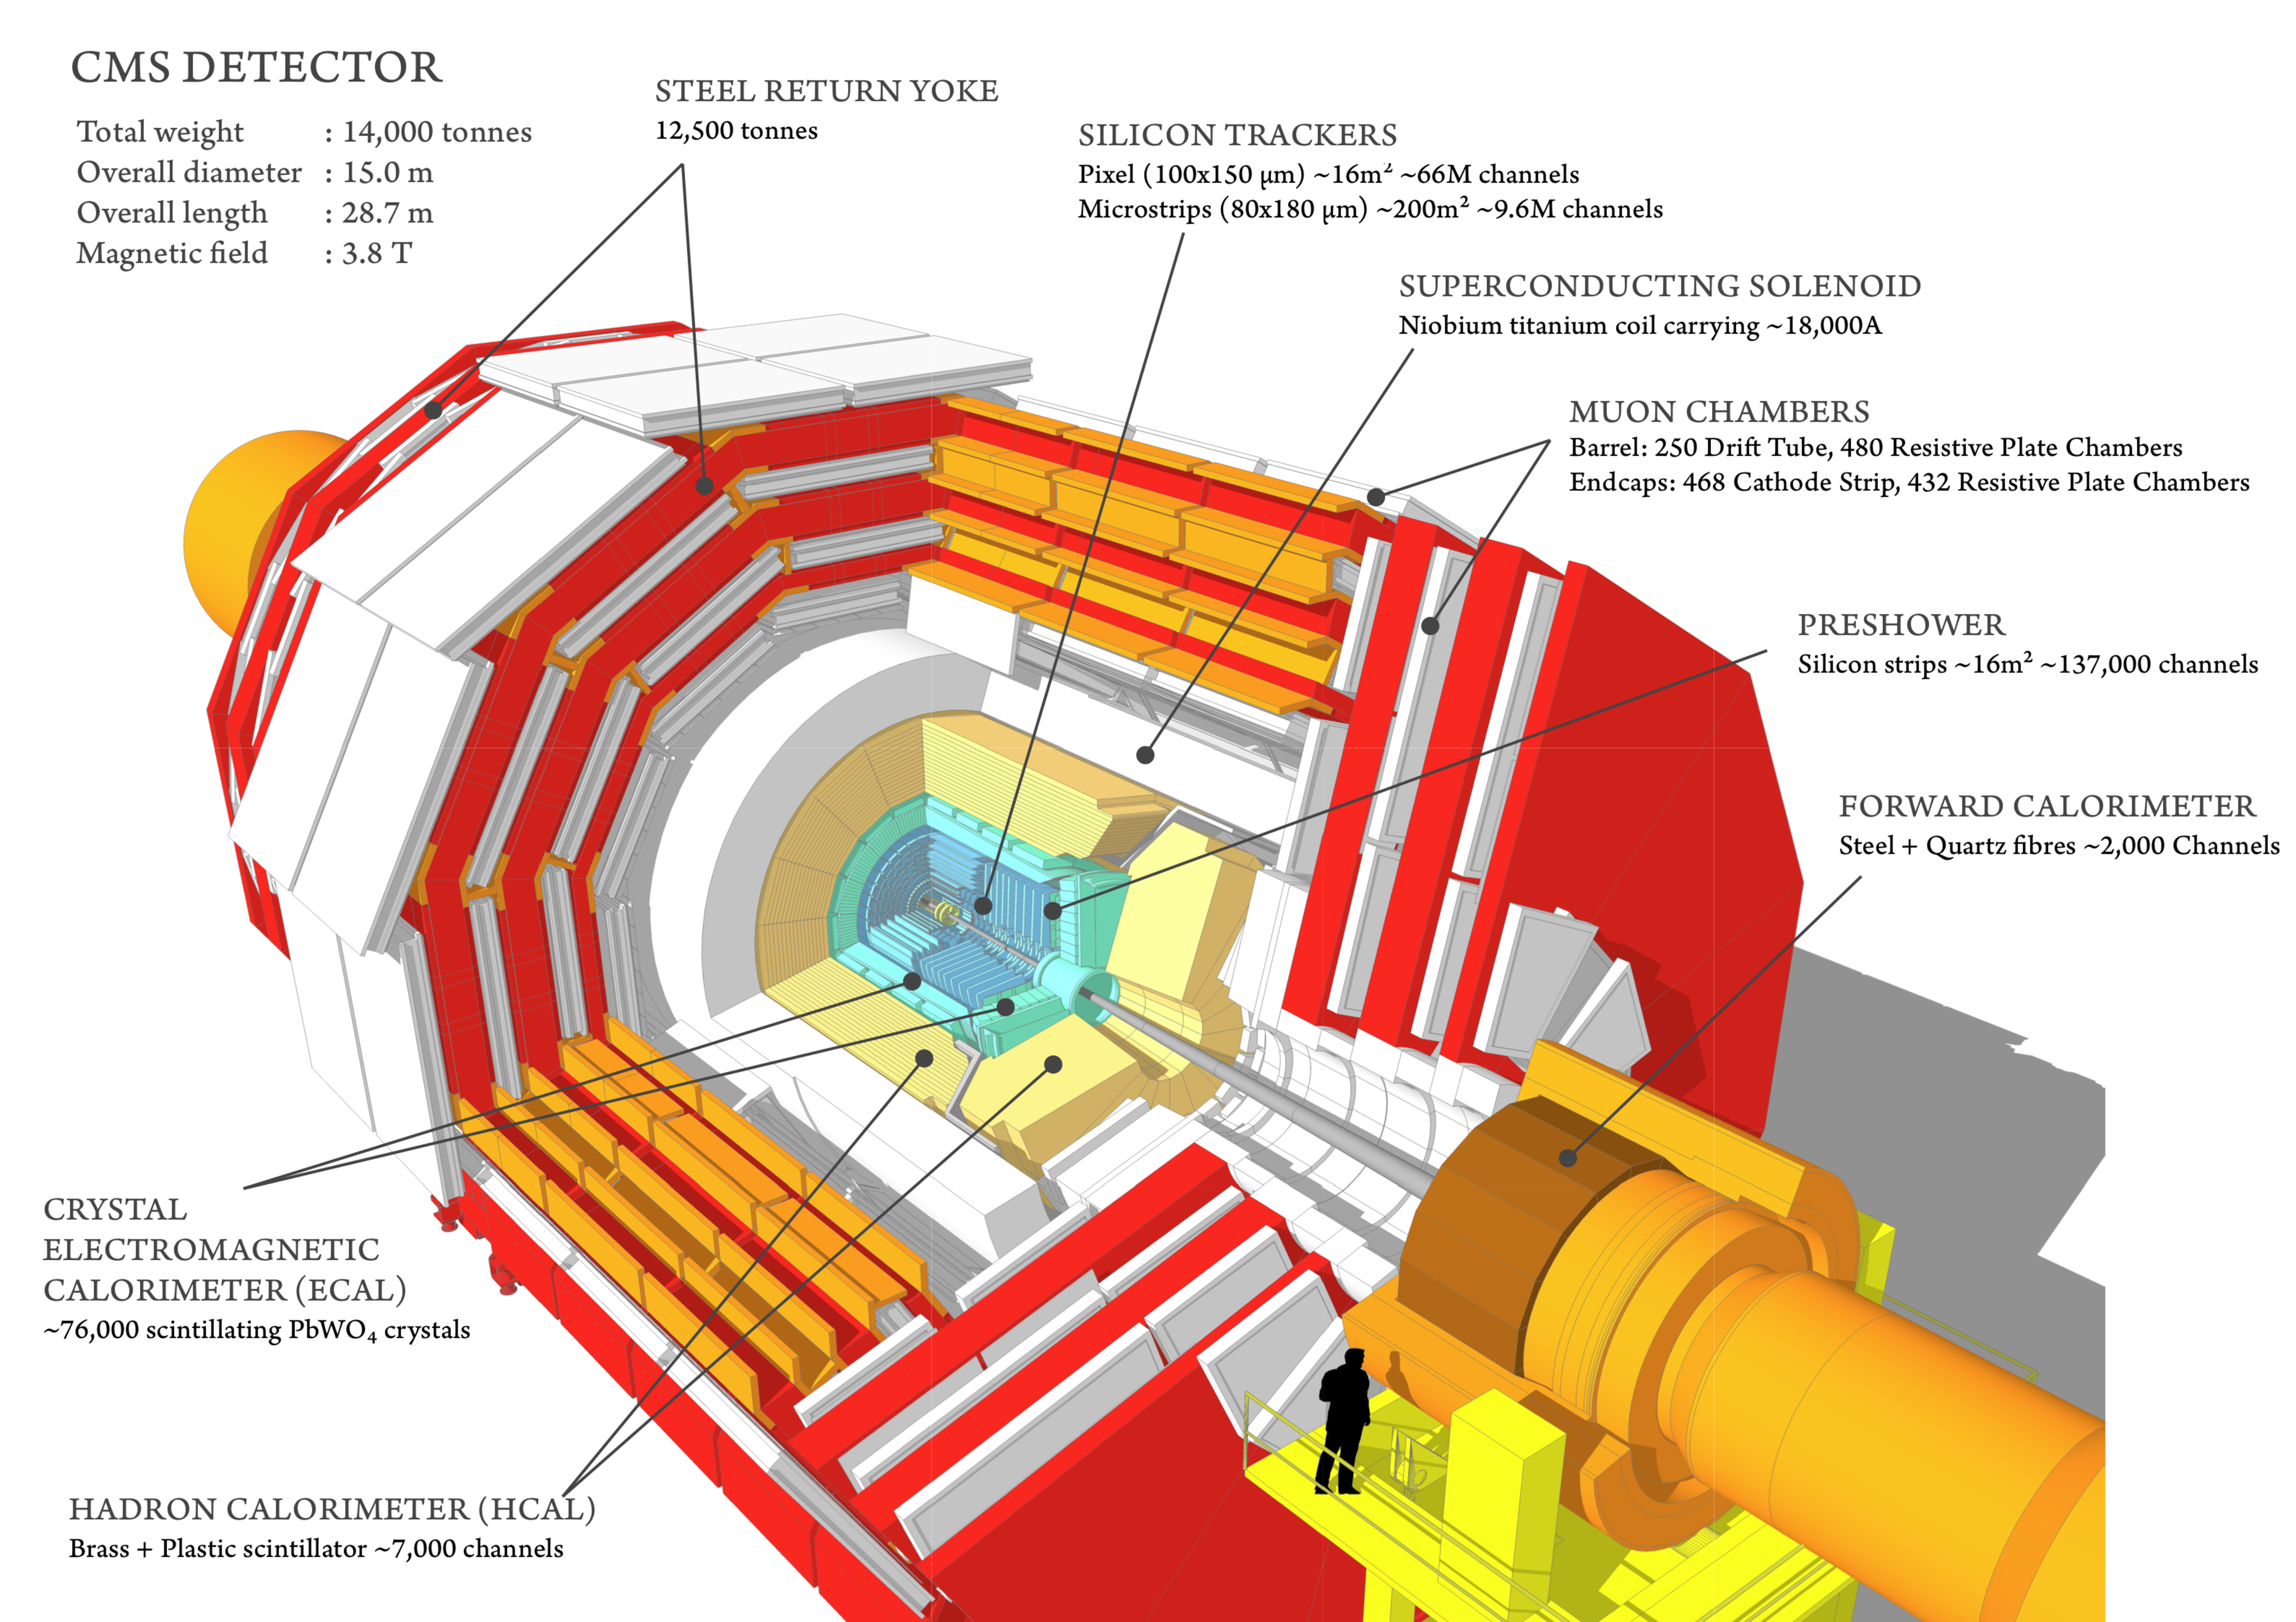
\includegraphics[width=0.7\textwidth]{images/CMS.pdf}
\caption{Schematic view of the CMS detector showing its sub-detectors.}\label{fig:CMS}
\end{figure}
\begin{figure}[htb]
\centering
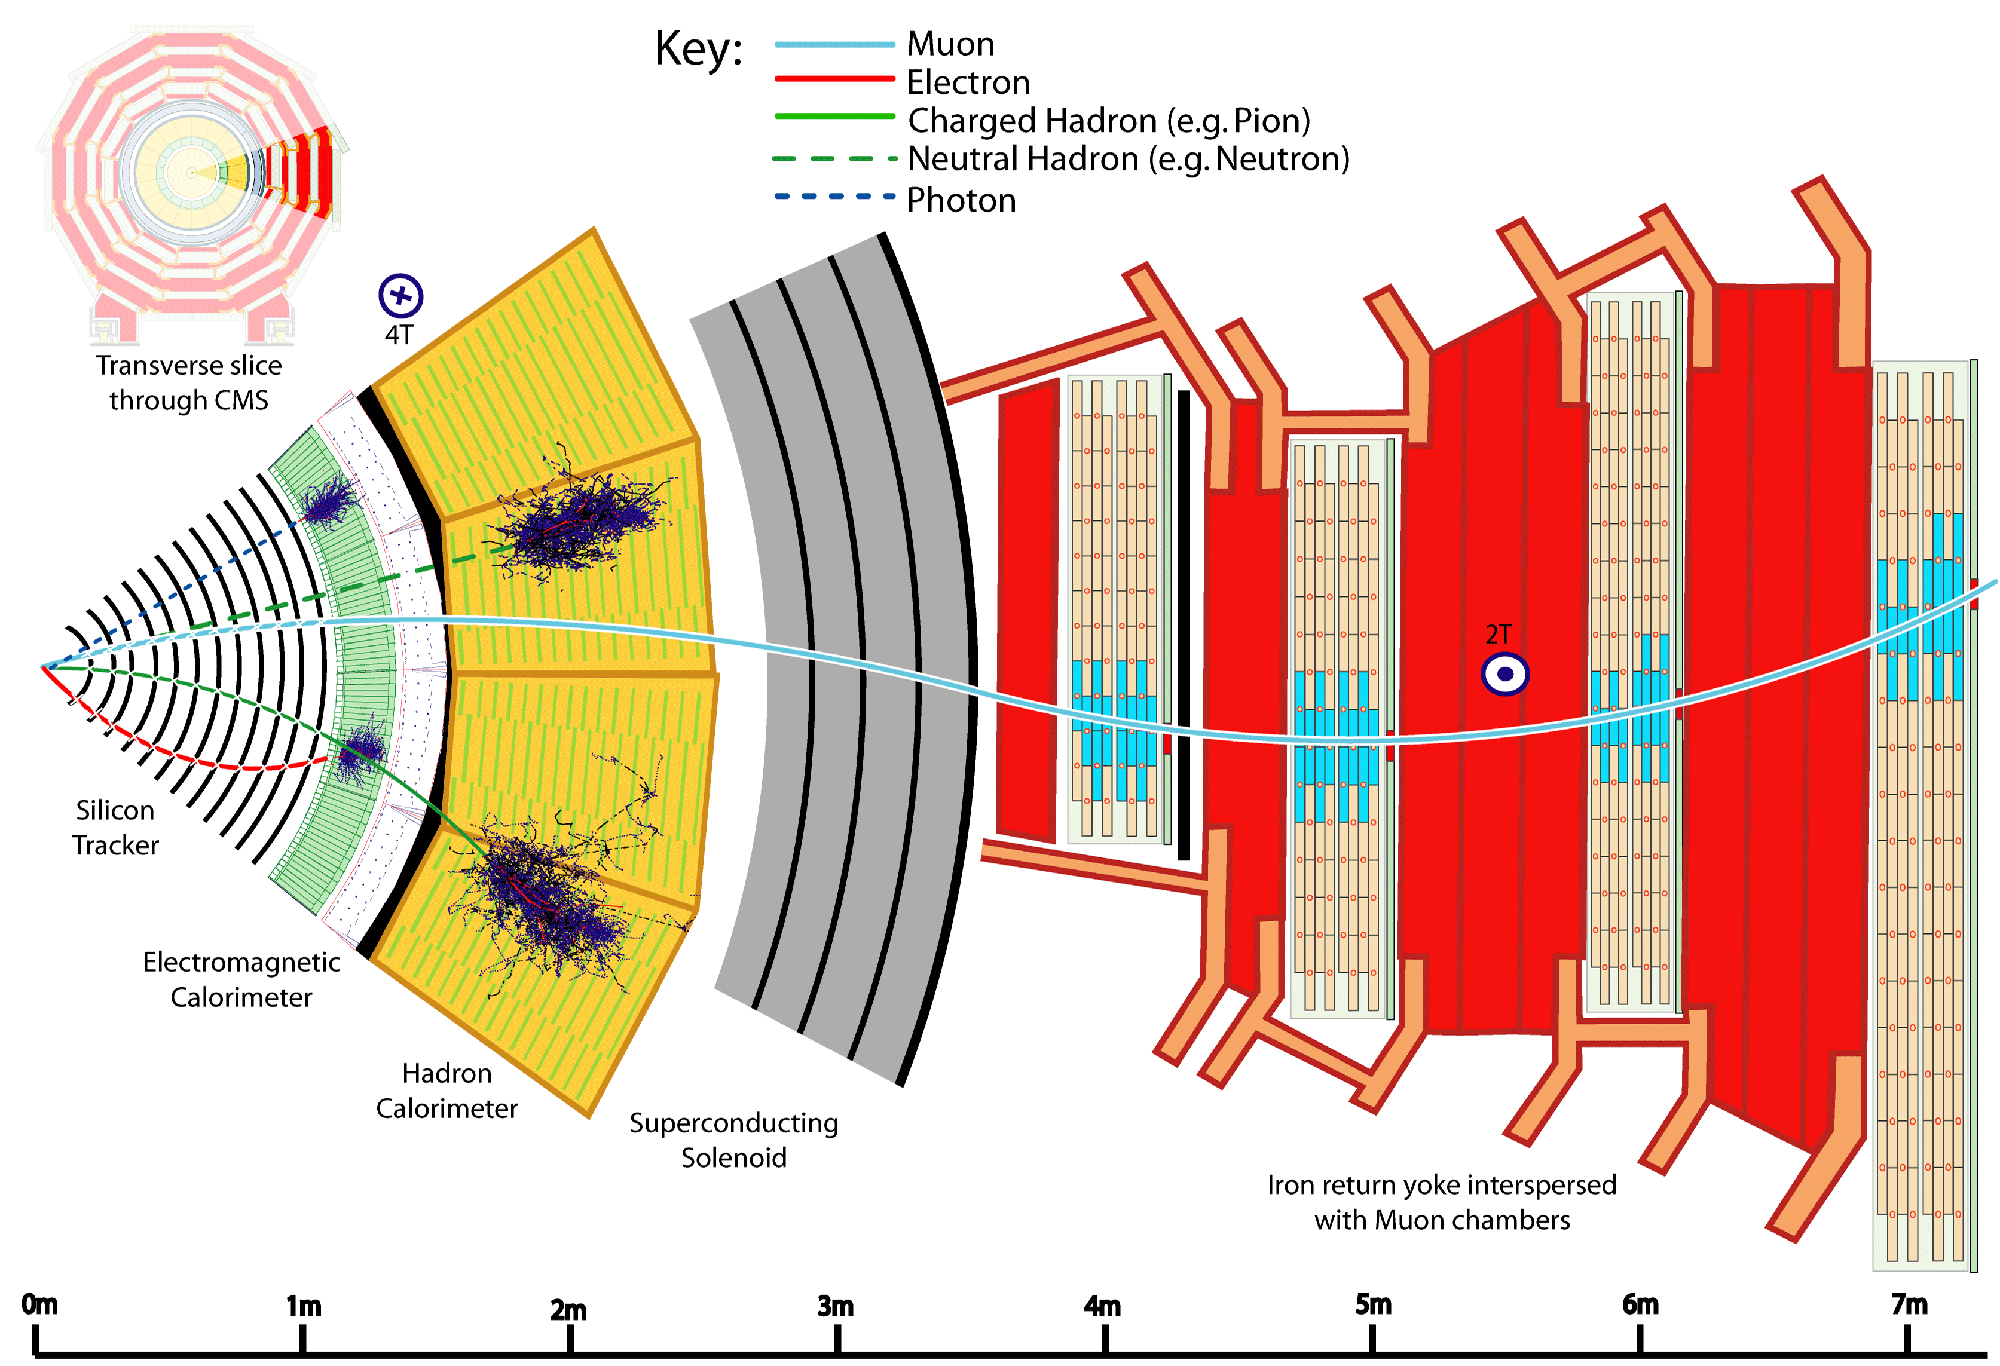
\includegraphics[width=0.7\textwidth]{images/CMSslice.png}
\caption{Schematic view of a slice of the CMS detector, showing the sub-detectors response to the passage of different types of particles.}\label{fig:CMSslice}
\end{figure}

In Fig.~\ref{fig:CMSslice} the response of the various CMS sub-detectors to the passage of different types of particles is sketched. In the following sections a brief description of each sub-detector is given.

%%%%%%%%%%%%%%%%%%%%%%%%%%%%%%%%%%%%%%%%%%%%%%%%%%%%%%%%%
\subsection{The solenoid}

The CMS magnet~\cite{CMSmagnet}, which contains the tracker, the electromagnetic and the hadronic calorimeters, is the biggest superconducting solenoid ever built. The solenoid can generate a magnetic field of $3.8$\,T in the internal bore, which has a diameter of 6\,m and a length of $12.5$\,m. The energy stored in the magnet is about $2.7$\,GJ at full current. The superconductor is made of four Niobium-Titanium layers and it is cooled down to about 4\,K through a liquid Helium cooling plant. In case of a quench, when the magnet loses its superconducting property, the energy is dumped to resistors within 200\,ms. The magnet return yoke of the barrel is composed of three sections along the $z$ axis; each one is split into 4 layers (holding the muon chambers in the gaps). Most of the iron volume is saturated or nearly saturated, and the field in the yoke is about half ($1.8$\,T) of the field in the central volume.

%%%%%%%%%%%%%%%%%%%%%%%%%%%%%%%%%%%%%%%%%%%%%%%%%%%%%%%%%
\subsection{The tracker}

The silicon tracker is the detector closest to the beam collision point. Its goal is the high resolution reconstruction of the trajectories of charged particles originating from the interaction point and the identification of the position of secondary vertices produced by particles with a short mean life time (in particular hadrons containing the b quark, that decay after few hundred of $\micron$). The events produced in the proton-proton collisions can be very complex and track reconstruction is an involved pattern recognition problem. Indeed, at the nominal instantaneous luminosity of operation, an average of about 20 pile-up events overlapping to the event of interest are expected, leading to about 1000 tracks to be reconstructed every 25\,ns. In order to make the pattern recognition easier, two requirements are fundamental:
\begin{itemize}
\item a low occupancy detector;
\item a large redundancy of the measured points (\emph{hits}) per track.
\end{itemize}
The first requirement is achieved building a detector with high granularity\footnote{The granularity of a detector is defined as the angular range ($\Delta\eta\times\Delta\phi$) that each individual element is able to resolve.}. The redundancy of the hits is instead achieved having several detecting layers, and is necessary to reduce the ambiguity on the assignment of the hits to a given track. Nevertheless, the amount of tracker material has to be as low as possible, in order to avoid compromising the measurement of the particle trajectory. An excessive amount of material would indeed deteriorate the measurement, mainly because of the increased probability of particle multiple scattering. The outer detectors such as ECAL would be influenced by the material as well, for example because of the increased probability for a photon to convert to an electron-positron pair in the tracker material. For this reasons, the tracker layers are limited in number and thickness.

The tracker comprises a large silicon strip detector with a small silicon pixel detector inside it. In the central $\eta$ region, the pixel tracker consists of three co-axial barrel layers at radii between $4.4$\,cm and $10.2$\,cm and the strip tracker consists of ten co-axial barrel layers extending outwards to a radius of $110$\,cm. Both sub-detectors are completed by endcaps on either
side of the barrel, each consisting of two disks in the pixel tracker, and three small plus nine large disks in the strip tracker. The endcaps extend the acceptance of the tracker up to $|\eta|<2.5$. A three-dimensional schematic view of the tracker is shown in Fig.~\ref{fig:tracker3D}, while in Fig.~\ref{fig:tracker2D} a pictorial representation of a slice of the tracker is displayed, showing the various layers of the sub-detectors.

\begin{figure}[htb]
\centering
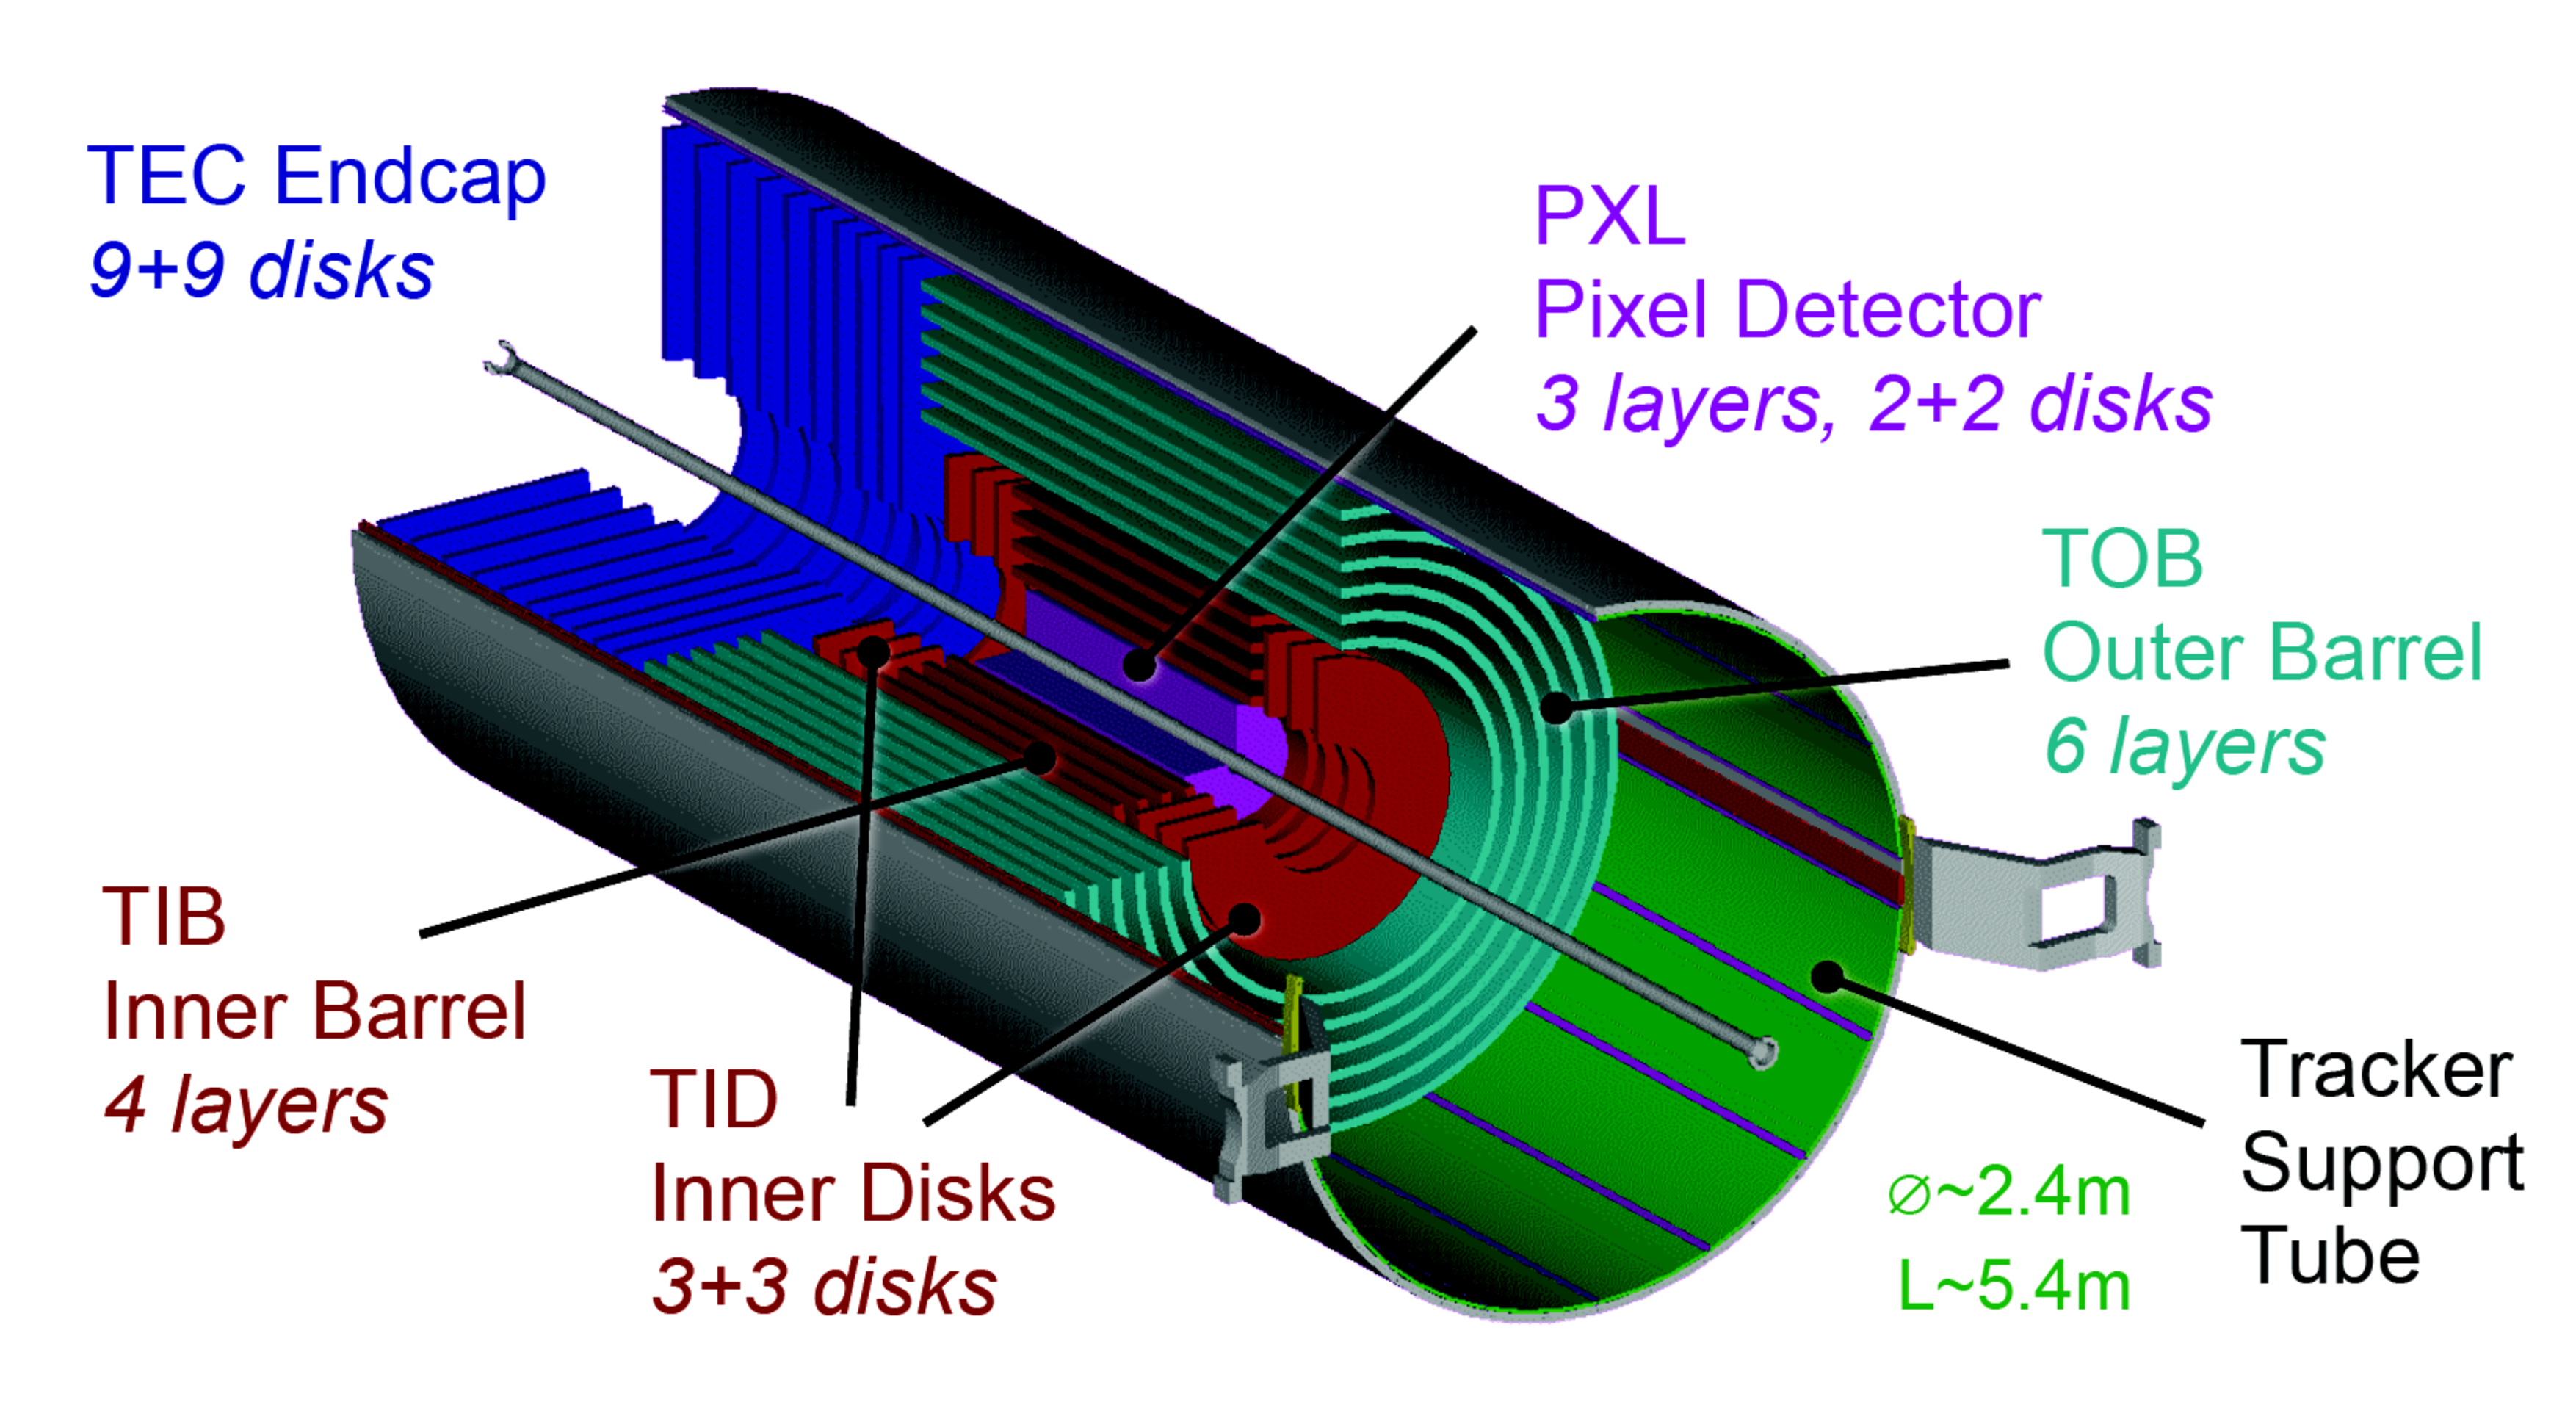
\includegraphics[width=0.6\textwidth]{images/tracker.pdf}
\caption{Three-dimensional schematic view of the CMS silicon tracker.}\label{fig:tracker3D}
\end{figure}
\begin{figure}[htb]
\centering
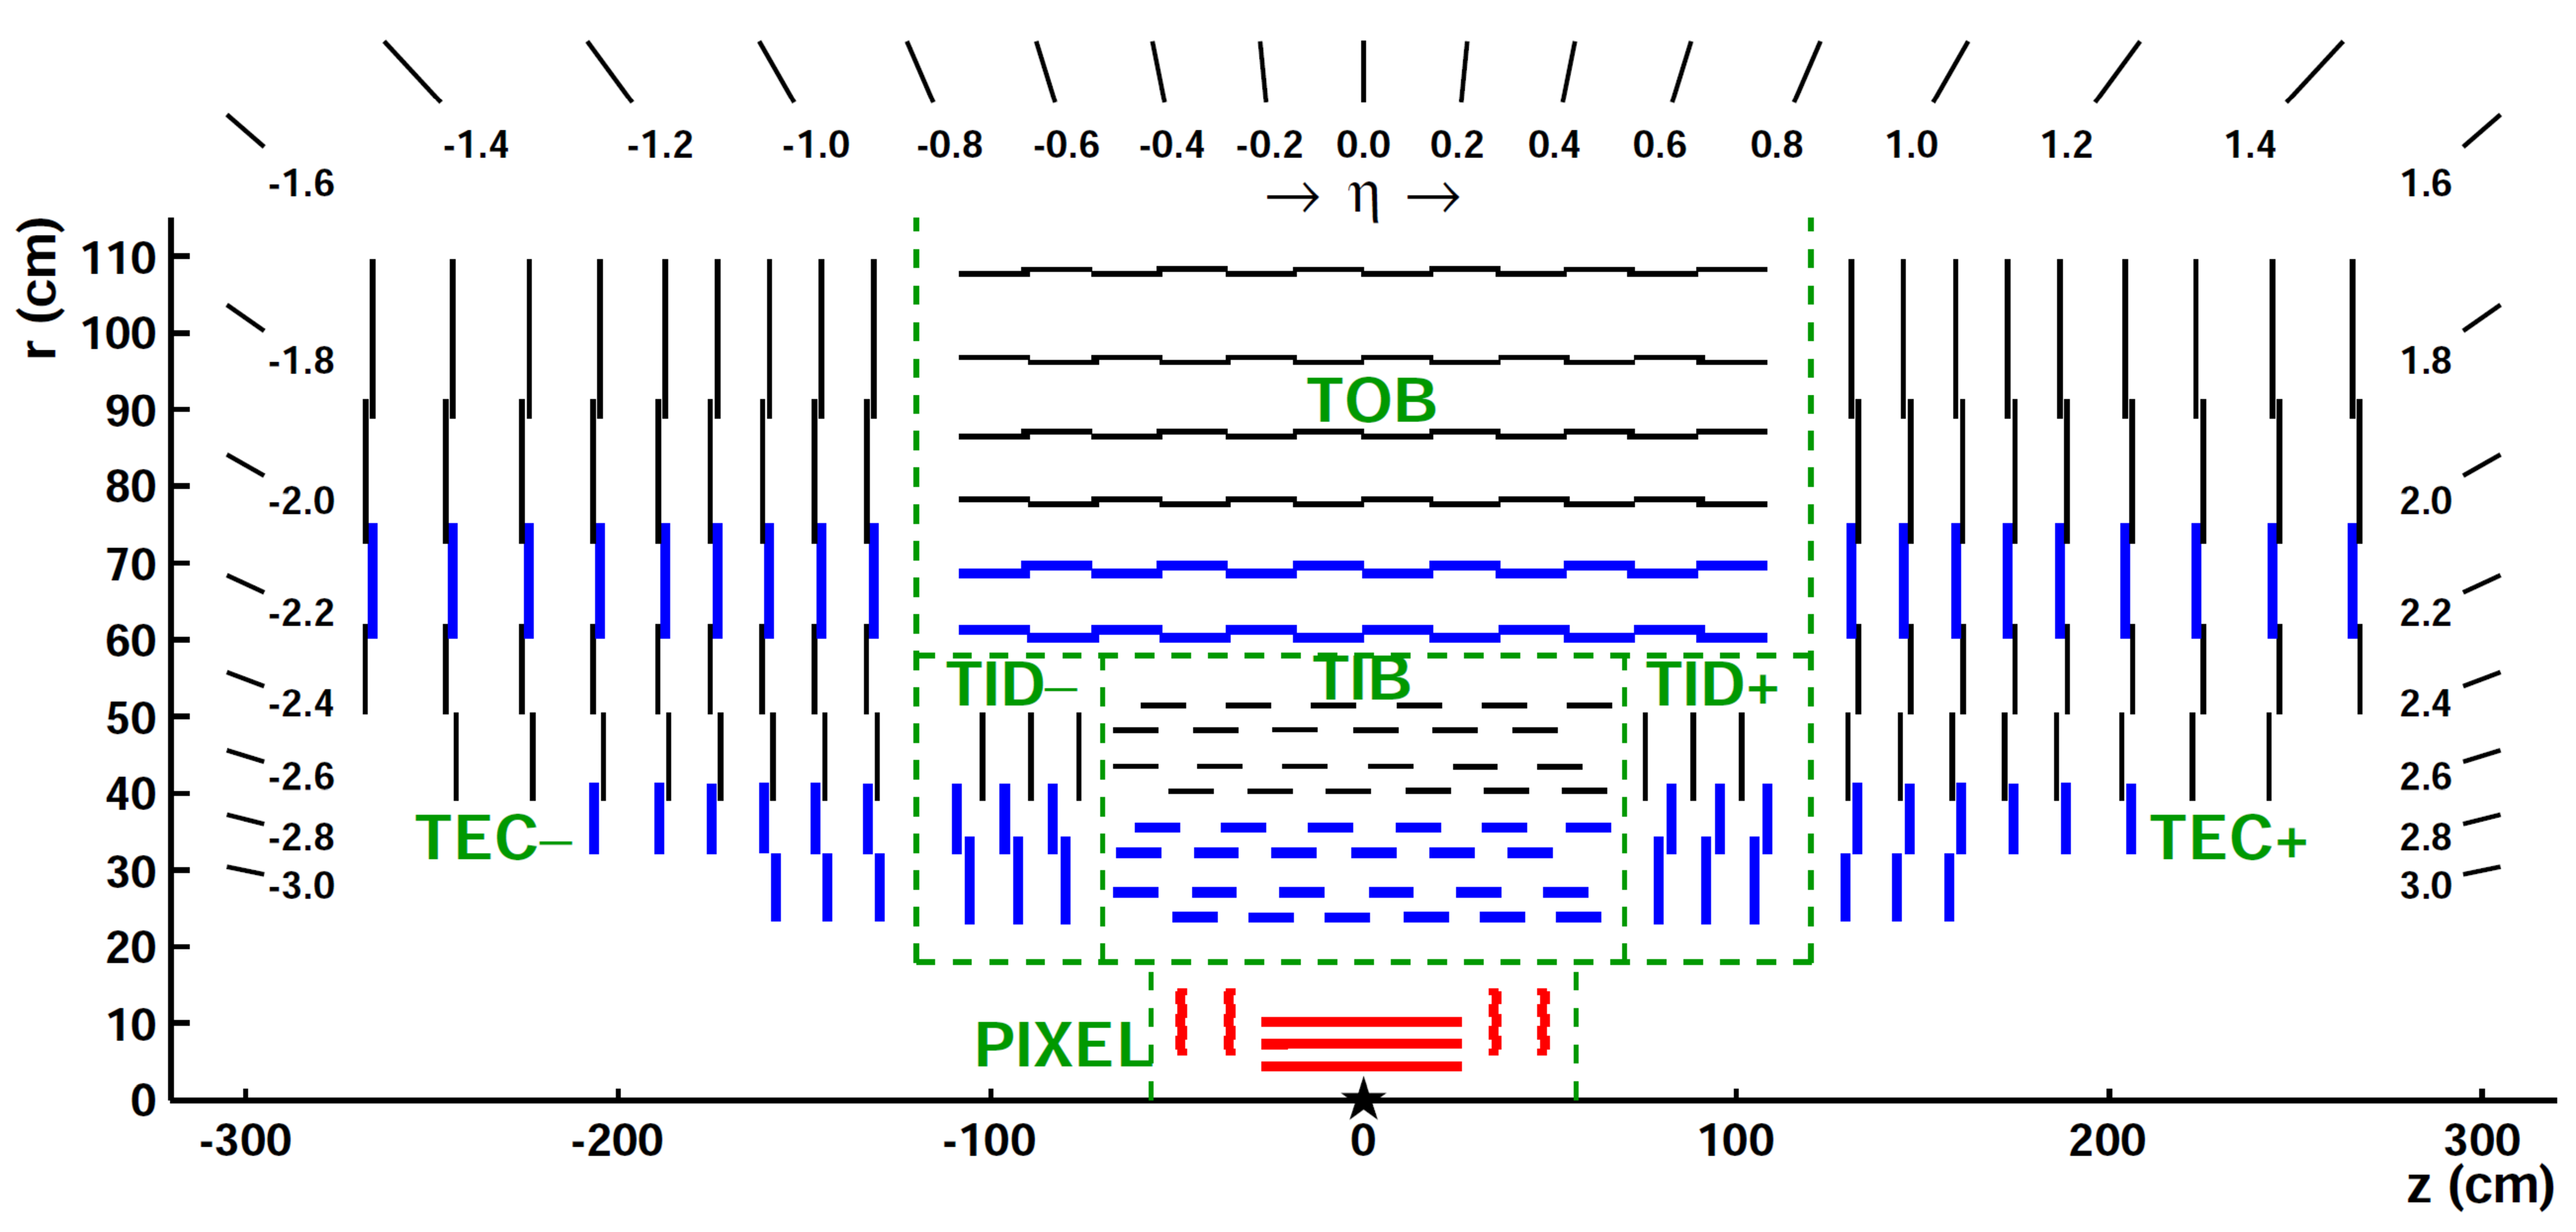
\includegraphics[width=0.8\textwidth]{images/tracker2D.pdf}
\caption{Pictorial view of a tracker slice in the r-z plane. Pixel modules are
shown in red, single-sided strip modules are depicted as black thin lines and
strip stereo modules are shown as blue thick lines.}\label{fig:tracker2D}
\end{figure}

The whole tracker has a cylindrical shape with a length of $5.8$\,m and a diameter of $2.5$\,m, with the axis aligned to the beams direction. The average number of hits per track is 12-14, allowing high reconstruction efficiency and low rate of fake tracks.

The material budget of the tracker as obtained from a simulation of the detector is shown in Fig.~\ref{fig:material_budget}, reported both in units of radiation length $t/X_0$ and in units of nuclear interaction length $t/\lambda_I$, as a function of $\eta$. The region $1 < |\eta| < 2$ exhibits a larger material budget due to the presence of cables and services.
\begin{figure}[htb]
\centering
\subfigure{
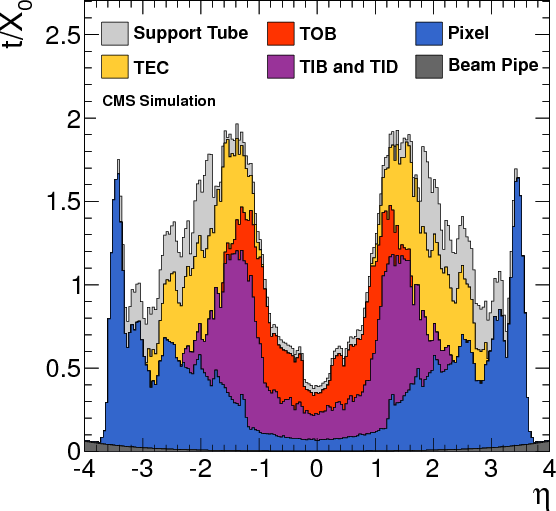
\includegraphics[width=0.45\textwidth]{images/materialBudget_X.png}
}
\subfigure{
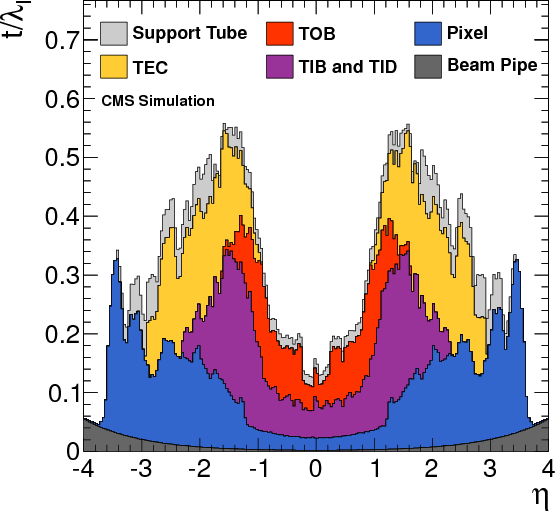
\includegraphics[width=0.45\textwidth]{images/materialBudget_lambda.png}
}
\caption{Total thickness $t$ of the tracker material expressed in units of $X_0$ (left) and $\lambda_I$ (right), as a function of $\eta$. The contribution to the total material budget of each part of the detector is shown.}\label{fig:material_budget}
\end{figure}

%%%%%%%%%%%%%%%%%%%%%%%%%%%%%%%%%%%%%%%%%%%%%%%%%%%%%%%%%
\subsubsection{The pixel detector}

The pixel detector, shown in Fig.~\ref{fig:pixel}, is mainly used as starting point in the CMS track reconstruction and is of fundamental importance for the reconstruction of primary and secondary vertices. 
\begin{figure}[htb]
\centering
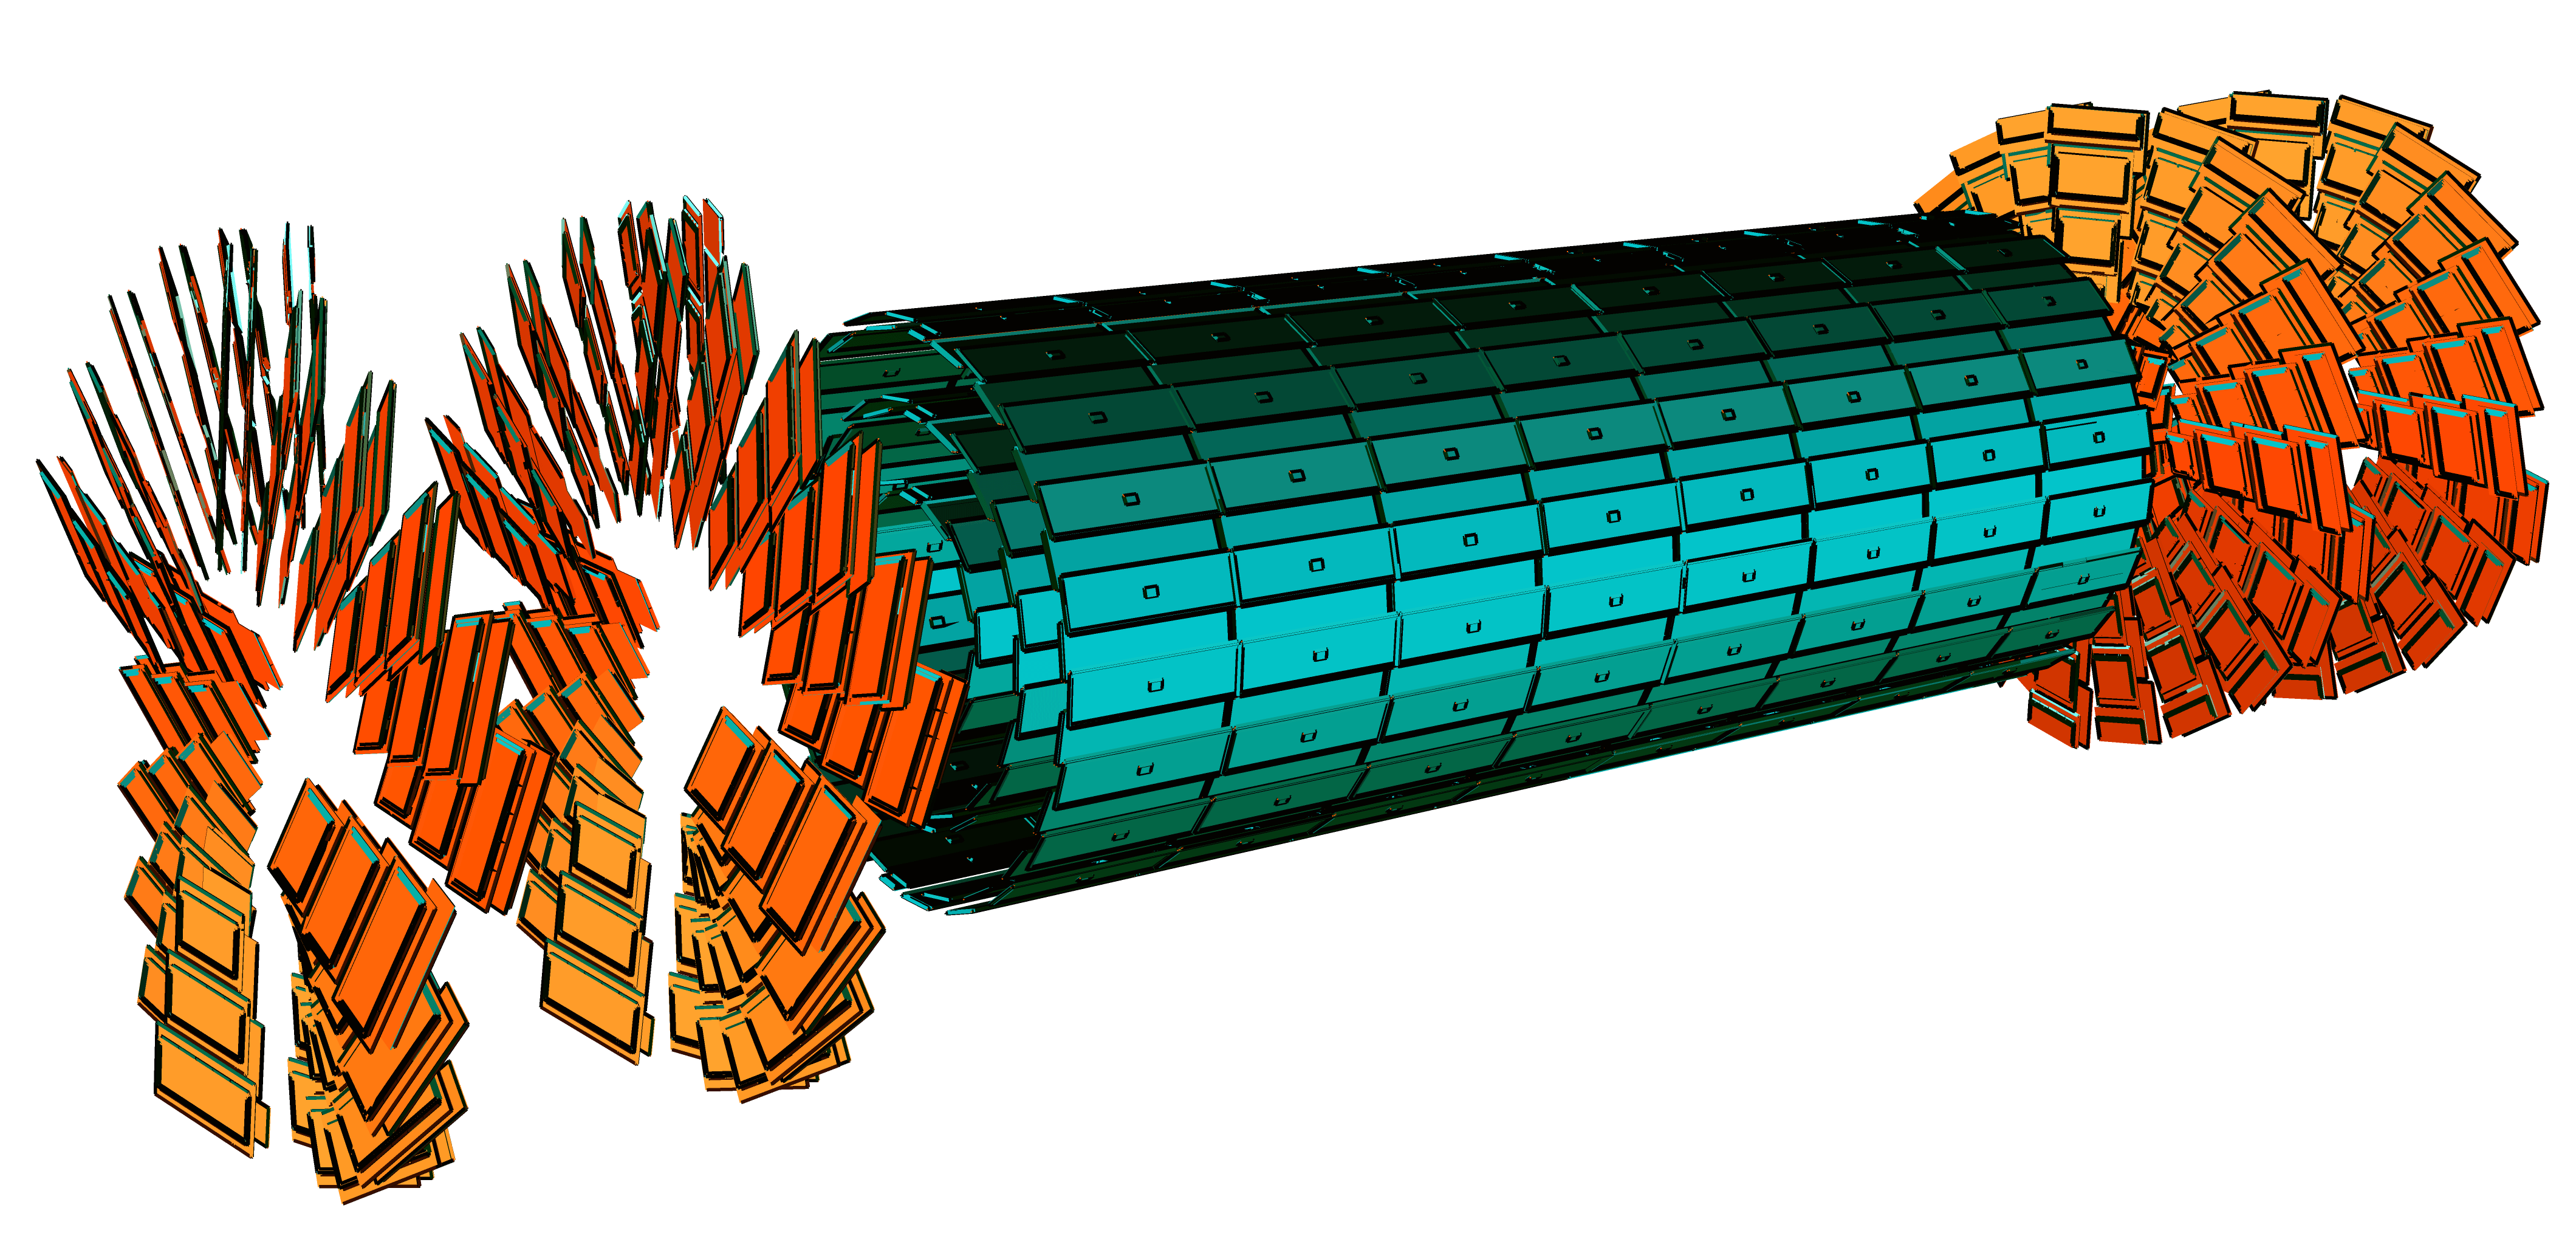
\includegraphics[width=0.5\textwidth]{images/pixel.png}
\caption{Schematic view of the CMS pixel detector.}\label{fig:pixel}
\end{figure}
The pixel detector is placed in the closest position to the collision point, where the amount of radiation is larger. It is placed in the region $|\eta|<2.5$ and consists of three cylindrical layers 53\,cm long in the barrel region, located at $r=4.4$, $7.3$ and $10.2$\,cm, and two pairs of endcap disks with radii between 6 and 15\,cm at $z=\pm34.5$ and $\pm46.5$\,cm, covering a total area of about $1\,\mathrm{m^2}$. The detector is composed of many modules, for a total of 768 in the barrel and 672 in the endcaps. Each endcap is composed of 24 segments, each one tilted with respect to the adjacent ones and containing 7 modules. Each module consists of several units which contain a highly segmented silicon sensor with a thickness of $250\,\micron$. In order to achieve an optimal vertex position resolution in both the $(r,\phi)$ and $z$ coordinates, a design with a rectangular pixel shape with an area of $150\times100\,\micron^2$ was adopted, with the $100\,\micron$ size oriented along the $(r,\phi)$ direction in the barrel region, and along the $z$ direction in the endcap region. The achievable hit reconstruction resolution is about 10--15$\,\micron$ in the barrel and $15\,\micron$ in the endcaps.

%%%%%%%%%%%%%%%%%%%%%%%%%%%%%%%%%%%%%%%%%%%%%%%%%%%%%%%%%
\subsubsection{The microstrip detector}

In this region of the detector the radiation flow is low enough to allow the use of a less segmented device, such as the silicon microstrip detector.
The microstrip tracker is composed of 15148 silicon modules, covering a total area of about $193\,\mathrm{m^2}$ with a total of 9.3 million strips. Two types of modules are installed: single sided modules consist of one sensor sticked onto a carbon fiber support together with the readout electronics, with the silicon strips laying along the $z$ direction in the barrel and along the $(r,\phi)$ direction in the endcaps. The other type of module, referred to as stereo-module, consists of two sensors sticked together back to back and tilted of a relative angle of 100\,mrad. This combination allows a three-dimensional measurement of the particle interaction point, providing the information along the $z$ direction. The whole microstrip tracker is $5.4$\,m long and extends up to $r=1.1$\,m. As the pixel detector, the microstrip detector consists of a barrel and an endcap region and is divided into four distinct parts, as shown in Fig.~\ref{fig:tracker2D}. The barrel is made up of the following parts:
\begin{itemize}
\item TIB (\emph{Tracker Inner Barrel}): it consists of four cylindrical coaxial layers, covering the region up to $|z|<65$\,cm. In this region the detectors have a thickness of $300\,\micron$ and the strips are separated by a variable pitch between 80 and $120\,\micron$. The first two layers are composed of stereo modules while the other layers have single-sided modules. Since the strips are oriented along the $z$ axis, the position resolution is more precise in the $(r,\phi)$ direction, about 23--34$\,\micron$, with respect to the $z$ direction, where a resolution of about $230\,\micron$ is obtained thanks to the stereo modules.
\item TOB (\emph{Tracker Outer Barrel}): it consists of six cylindrical coaxial layers, placed in the region $55\,\mathrm{cm} < r < 65\,\mathrm{cm}$ and $|z|<110$\,cm. Stereo modules are mounted on the two inner layers. Since the density of particles passing through this region is lower with respect to the TIB, the pitch between the strips is larger (120--180$\,\micron$) and the strips are longer ($190$\,mm). The spatial resolution varies in the range 25--52$\,\micron$ in the $(r,\phi)$ direction, and is about $530\,\micron$ in the $z$ coordinate for the stereo modules.
\end{itemize}
The endcaps are also made up of two parts:
\begin{itemize}
\item TID (\emph{Tracker Inner Disk}): it consists of six disks, three per side, placed orthogonally with respect to the beam axis, between the TIB and the TOB. The modules are positioned in a ring shape, with the strips oriented in the radial direction, and are alternately placed on the internal and external side of the disk. The two innermost rings of the TID are equipped with stereo modules. The thickness of the silicon is $300\,\micron$.
\item TEC (\emph{Tracker EndCap}): each one of the two TEC is made of nine disks which extend to the region $120\,\mathrm{cm} < |z| < 280\,\mathrm{cm}$. Each disk is divided into 8 slices in each of which a number ranging from 4 to 7 modules are mounted in a ring shape, depending on the position along $z$. Also in this case the modules are alternately mounted on the internal and external side of the disk, with the strips radially oriented. On the two innermost rings and on the fifth one the stereo modules are installed to measure the $z$ coordinate. The thickness of the sensors range between 300 and $500\,\micron$ depending on the disk.
\end{itemize}
The tracker is operated at low temperature in order to reduce those radiation damage induced effects that have a temperature dependence, such as the increase of the leakage current and the long-term increase of the depletion voltage (also called reverse annealing)\footnote{The tracker in Run 1 was operated at a temperature of $+4^{\circ}$C, but during the Long Shutdown 1 a new cooling dry gas plant has been installed and the tracker is now operating at the lower temperature of $-15^{\circ}$C.}.

The alignment of the tracker modules is very important to obtain a high spatial resolution. Deviations are caused by assembly inaccuracy, deformations due to cooling and stress from the magnetic field. Therefore, three methods are used for the tracker alignment.
The geometry was determined during the assembly to an accuracy of 80 to $150\,\micron$. An infrared laser system is used for continuous monitoring of the position of selected tracker modules. The final alignment is done with tracks from well known physics processes, e.g. cosmic muons or muon pairs from the $J/\Psi$, $\Upsilon$ or Z decays.

%%%%%%%%%%%%%%%%%%%%%%%%%%%%%%%%%%%%%%%%%%%%%%%%%%%%%%%%%
\subsection{The electromagnetic calorimeter (ECAL)}

The main function of an electromagnetic calorimeter is to identify electrons and photons and to accurately measure their energy. The CMS electromagnetic calorimeter (ECAL)~\cite{ecal,Bloch:581342}, shown in Fig.~\ref{fig:ecal}, is a hermetic homogeneous calorimeter with cylindrical geometry, composed of many scintillating crystals of lead tungstate ($\mathrm{PbWO_4}$) with a truncated pyramidal shape. As the other detectors it consists of two parts, the ECAL barrel (EB), which contains $61200$ crystals, and two endcaps (EE) containing 7324 crystals each one.

\begin{figure}[htb]
\centering
\subfigure[$r$--$z$ view of an ECAL sector.]{
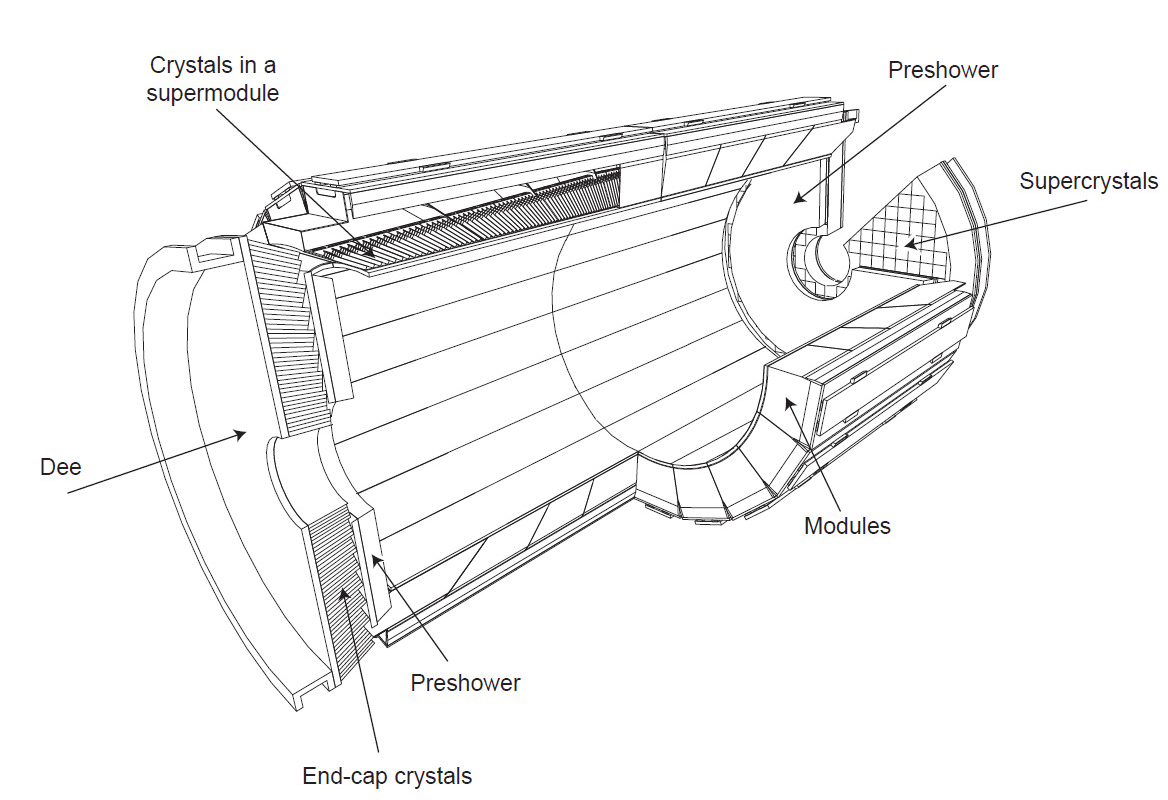
\includegraphics[width=0.45\textwidth]{images/ecal.png}
}
\subfigure[ECAL three-dimensional view.]{
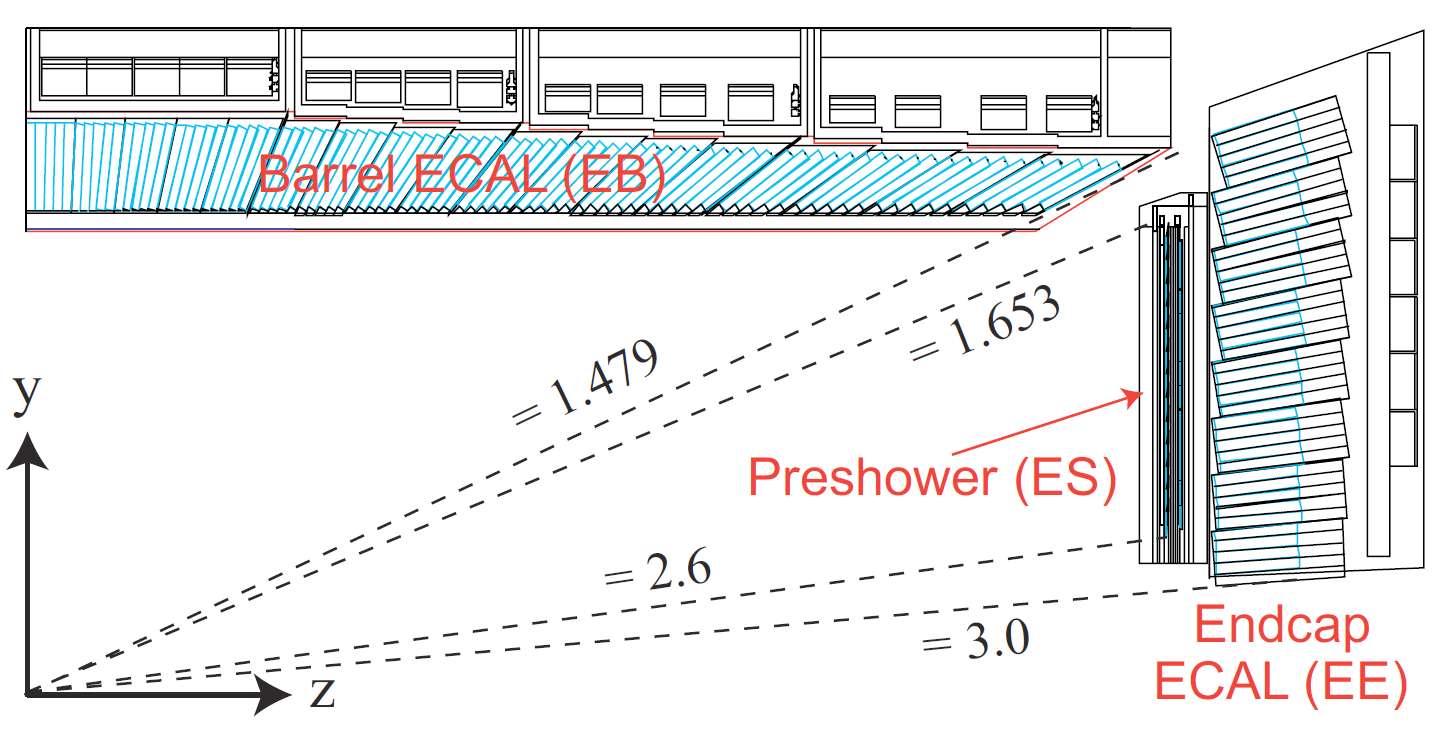
\includegraphics[width=0.45\textwidth]{images/ecalyz.png}
}
\caption{Schematic representation of the CMS electromagnetic calorimeter.}\label{fig:ecal}
\end{figure}

The characteristics of the $\mathrm{PbWO_4}$ crystals make them an appropriate choice for operation at LHC. The high density ($\rho=8.3\,\mathrm{g/cm^3}$), short radiation length ($X_0 = 0.89\,\mathrm{cm}$) and small Moli\`ere radius\footnote{The Moli\`ere radius $R_M$ characterizes the transverse development of an electromagnetic shower in a calorimeter. On average 90\% of the energy deposited by a shower is contained inside a cylinder with radius $R_M$.} ($2.2$\,cm) allow to build a compact and high granularity calorimeter. Another advantage of this material is the radiation hardness and the fast scintillation decay time ($\tau = 10$\,ns), that permits to collect about 80\% of the produced light within the 25\,ns interval between two consecutive bunch crossings. The main drawbacks of this material are the low light yield ($\sim 10~\mathrm{photoelectrons/MeV}$) and the strong dependence on the operating temperature, that makes it necessary to keep the crystals at a stabilized temperature ($18\degree$C).

The crystals are grouped into $5\times5$ matrices called \emph{towers}. The barrel has an inner radius of 129\,cm, a length of 630\,cm and extends in the region $|\eta|<1.479$. The crystals in the barrel have the following dimensions: $22\times22\,\mathrm{mm^2}$ at the front face, $26\times26\,\mathrm{cm^2}$ at the rear face, and a length of 23\,cm, corresponding to $25.8 X_0$, and are mounted in a quasi-projective geometry, in order to have the long side tilted by $3\degree$ with respect to the direction pointing to the interaction point, both in the $\eta$ and $\phi$ coordinates. This is done to avoid the empty spaces between adjacent crystals to be aligned with the direction pointing to the interaction point. The granularity of the EB is about $1\degree$.
Avalanche photodiodes (APDs) are used as photodetectors connected with the crystals in the barrel region.

Each endcap covers the region $1.479 < |\eta| < 3$ and is formed by two semicircular aluminium halves called \emph{dees}. Crystals in endcaps have a length of 22\,cm, a frontal area equal to $28.6\times 28.6\,\mathrm{mm^2}$ and a rear surface of $30\times 30\,\mathrm{mm^2}$. In the endcaps the crystals are arranged in a $\eta$--$\phi$ simmetry. The photodetectors used to collect the light produced in the endcap crystals are single stage vacuum phototriodes (VPTs), because this region experiences a rather high particle flux and VPTs are more robust against radiation damages with respect to APDs. A preshower system is installed in front of the ECAL endcaps in order to separate the showers produced by a primary $\gamma$ from those produced by forward emitted $\pi^0$. This detector, which covers the region $1.653<|\eta|<2.6$, is a sampling calorimeter consisting of two lead disks ($2 X_0$ and $1 X_0$ thick respectively) that initiate the electromagnetic shower from incoming photons or electrons, with silicon strip sensors after each disk, which measure the deposited energy as well as the shower transverse profile.

The energy resolution of a homogeneous calorimeter can be expressed by the sum in quadrature of three terms, as shown in the following formula:
\begin{equation}
\left(\frac{\sigma_E}{E}\right)^2 = \left(\frac{a}{\sqrt{E}}\right)^2 + \left(\frac{b}{E}\right)^2 + c^2
\end{equation}

The stochastic term $a$ dominates at low energies: it includes the contribution of statistical fluctuations in the number of generated and collected photoelectrons. This term takes into account the crystal light emission, the light collection efficiency and the photodetector quantum efficiency\footnote{The quantum efficiency is the ratio between the number of collected electron-hole pairs (or photoelectrons) and the number of photons incident on the photodetector.}. The noise term $b$ includes the contributions of pile-up events and electronic noise, both due to the photodetector and preamplifier. These contributions depend on $\eta$ and on the LHC operational luminosity.
The constant term $c$, dominant at high energies, takes into account several contributions. The most relevant are the non-uniformity of the longitudinal light collection, the intercalibration errors and the leakage of energy from the rear side of the crystal. The EB resolution for electrons was measured using test beams to be:
\begin{equation}
\left(\frac{\sigma_E}{E}\right)^2 = \left(\frac{2.8\%\,\mathrm{GeV^{1/2}}}{\sqrt{E}}\right)^2 + \left(\frac{12\%\,\mathrm{GeV^{1/2}}}{E}\right)^2 + (0.3\%)^2 \quad,
\end{equation}
where $E$ is the energy measured in GeV.

%%%%%%%%%%%%%%%%%%%%%%%%%%%%%%%%%%%%%%%%%%%%%%%%%%%%%%%%%
\subsection{The hadron calorimeter (HCAL)}

The hadron calorimeter (HCAL)~\cite{hcal} is used together with ECAL to make a complete calorimetric system for the jet energy and direction measurement. Moreover, thanks to its hermetic structure, it can measure the energy imbalance in the transverse plane, \MET, a typical signature of non interacting particles such as neutrinos. The HCAL is a sampling calorimeter covering the region $|\eta|<5$. As shown in Fig.~\ref{fig:hcal}, it is divided in four sub-detectors: HB (\emph{Barrel Hadronic Calorimeter}), located in the barrel region inside the solenoid, extending up to $|\eta|<1.4$; HE (\emph{Endcap Hadronic Calorimeter}), placed in the endcaps region inside the magnet, covering the region $1.3 < |\eta| < 3$ and partially overlapping with the HB coverage; HO (\emph{Outer Hadronic Calorimeter}), also known as \emph{tail-catcher}, placed along the inner wall of the magnetic field return yoke, just outside of the magnet; HF (\emph{Forward Hadronic Calorimeter}), a sampling calorimeter consisting of quartz fibers sandwiched between iron absorbers,
formed by two units placed in the very forward region ($3<|\eta|<5$) outside the magnetic coil. The quartz fibers emit Cherenkov light with the passage of charged particles and this light is detected by radiation resistant photomultipliers.
\begin{figure}[htb]
\centering
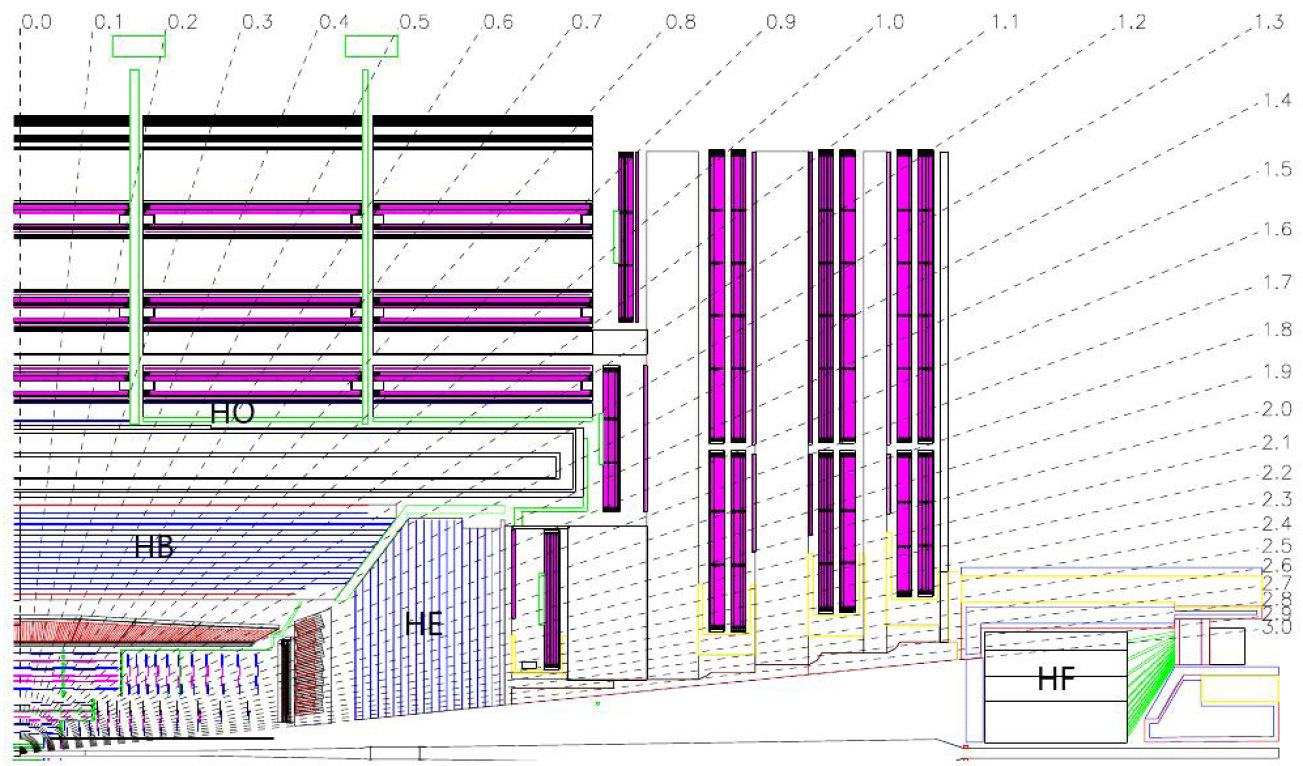
\includegraphics[width=0.6\textwidth]{images/hcal.png}
\caption{Longitudinal view of the CMS detector showing the HCAL sub-detectors.}\label{fig:hcal}
\end{figure}
In order to maximize particle containment for a precise missing transverse energy measurement, the amount of absorber material was maximized, reducing therefore the amount of the active material. Since HCAL is mostly placed inside the magnetic coil, a non-magnetic material like brass was chosen as absorber. HB and HE are therefore made with 5\,cm brass absorber layers interleaved with 3.7\,mm plastic scintillators. The scintillation light is collected by wavelength shifting (WLS) fibres and read out by hybrid photodiodes (HPD). The granularity of the calorimeter is $\Delta\eta\times\Delta\phi = 0.087 \times 0.087$ for $|\eta|<1.6$ and $\Delta\eta\times\Delta\phi \approx 0.17 \times 0.17$ for $|\eta|\geq1.6$. HO is made of 5 rings installed in the wheel that compose the return yoke and is divided in 12 sectors, each one covering a $30\degree$ angle in $\phi$. It consists of scintillating layers, with the same granularity as HB, and the solenoid coil is used as an additional absorber to increase the effective depth of the calorimeter in the barrel region, which is extended up to $11.8\,\lambda_I$, thus improving the energy resolution.

The energy resolution in the different regions of HCAL can be parametrized using a stochastic and a constant term, as follows:
\begin{equation}
\begin{split}
\left(\frac{\sigma_E}{E}\right)^2 &= \left(\frac{90\% \mathrm{GeV}^{1/2}}{\sqrt{E}}\right)^2 + \left(4.5\%\right)^2 \qquad \mathrm{in~ the~ barrel/endcap}\quad,\\
\left(\frac{\sigma_E}{E}\right)^2 &= \left(\frac{172\% \mathrm{GeV}^{1/2}}{\sqrt{E}}\right)^2 + \left(9\%\right)^2 \qquad \mathrm{in~ the~ HF}\quad,
\end{split}
\end{equation}
where $E$ is expressed in GeV.


%%%%%%%%%%%%%%%%%%%%%%%%%%%%%%%%%%%%%%%%%%%%%%%%%%%%%%%%%
\subsection{The muon system}\label{sec:muonsyst}
The CMS muon system~\cite{muon} is dedicated to the identification and measure of high \pt muons, in combination with the tracker. The system is placed outside the magnetic coil, embedded in the return yoke, to fully exploit the 1.8\,T return flux.
\begin{figure}[htb]
\centering
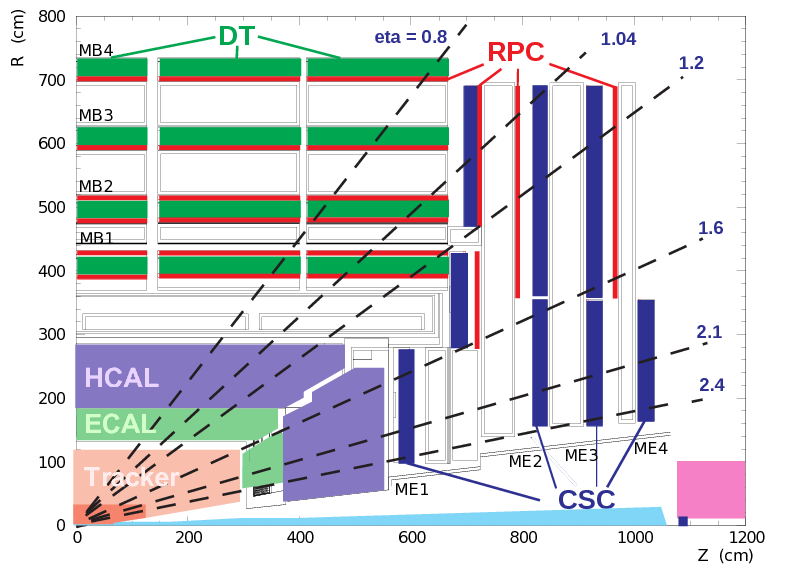
\includegraphics[width=0.5\textwidth]{images/muonsyst.png}
\caption{Schematic view of a quadrant of the CMS muon system.}\label{fig:muonsyst}
\end{figure}
As shown in Fig.~\ref{fig:muonsyst}, the system consists of three types of independent gaseous particle detectors:
\begin{itemize}
\item \emph{Drift Tubes} (DT) are placed in the barrel region, where the occupancy is relatively low ($< 10\,\mathrm{Hz/m^2}$);
\item \emph{Cathode Strip Chambers} (CSC) are installed in the endcaps, where the occupancy is higher ($> 100\,\mathrm{Hz/m^2}$);
\item \emph{Resistive Plate Chambers} (RPC) are placed both in the barrel and endcaps.
\end{itemize}
The DT system is placed in the region of the barrel with $|\eta|<1.2$, where the magnetic field is sufficiently weak and homogeneous. Along the longitudinal direction, the barrel region is divided in 5 wheels, which are subdivided in 12 sectors covering a $30\degree$ azimuthal angle each. The wheels are composed of 4 concentric rings of chambers, called \emph{stations}, interspersed in the layers of the iron return yoke, and each one formed by 12 DT chambers. The basic element of the DT system is a rectangular drift tube cell with a transverse size of $13\times42\,\mathrm{mm^2}$ and a variable length from 2 to 4\,m. The chambers are filled with a gas mixture of Ar (85\%) and $\mathrm{CO_2}$ (15\%) and are grouped in the radial direction to form detection layers. Groups of four layers form a \emph{superlayer}. In each superlayer two chambers have anode wires parallel to the beam axis and two have perpendicular wires, thus providing two measurements of the $(r,\phi)$ coordinate and two measurements of the $z$ coordinate of the track hit position.
\begin{figure}[htb]
\centering
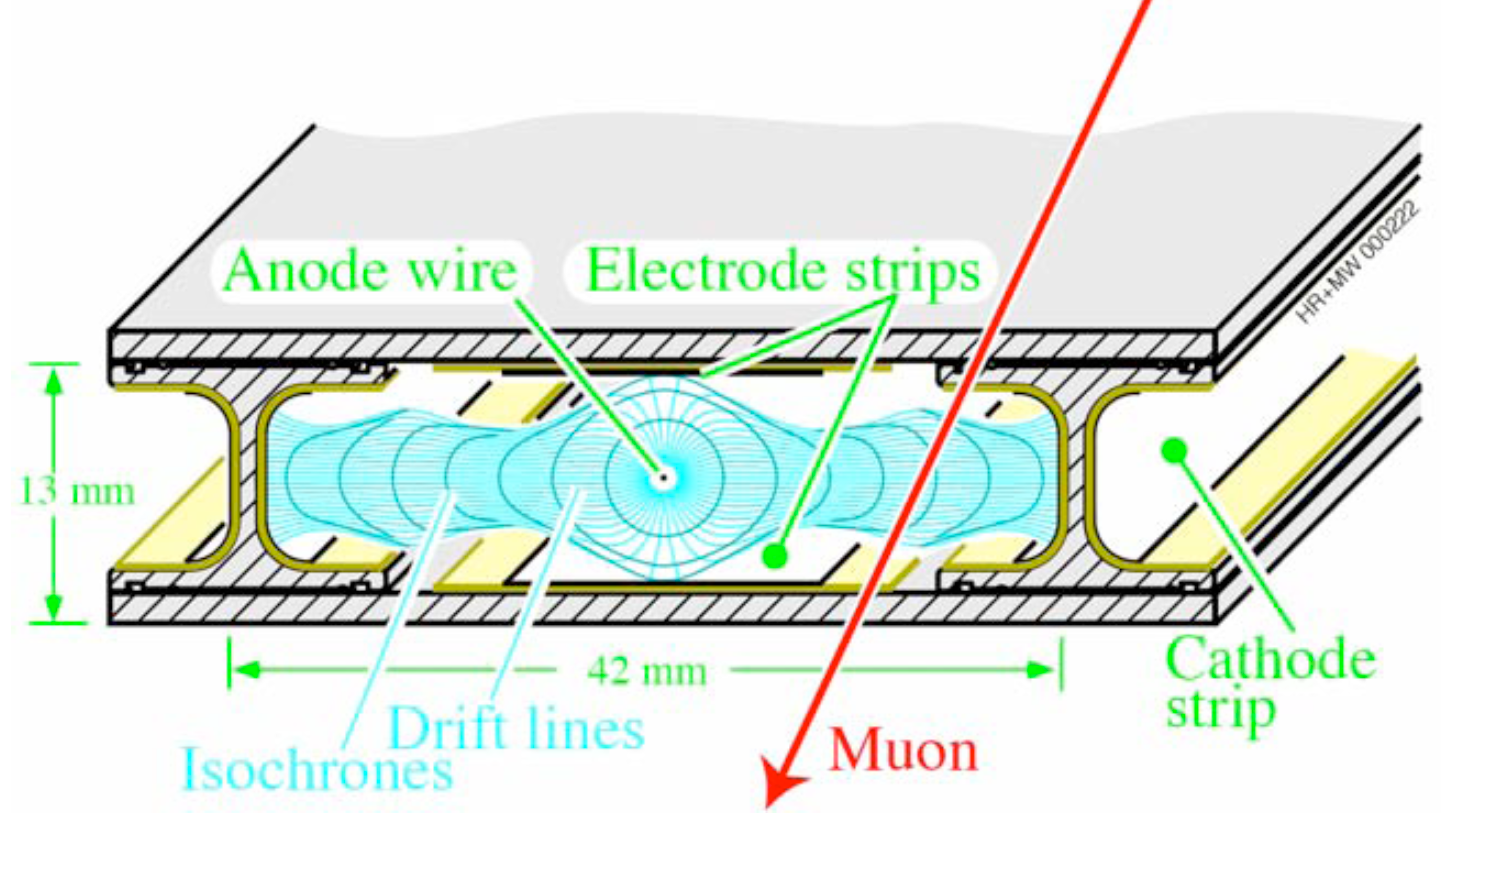
\includegraphics[width=0.5\textwidth]{images/drifttube.png}
\caption{Schematic representation of a drift tube chamber, showing the drift lines in presence of magnetic field.}\label{fig:dt}
\end{figure}
As shown in Fig.~\ref{fig:dt}, each chamber is made of a stainless steel anode wire between two parallel aluminium plates with ``I'' shaped spacer cathodes, isolated from the aluminium plates with polycarbonate plastic. The hit resolution is about $100\,\micron$ in both $(r,\phi)$ and $(r,z)$ directions.

In the endcaps, the high and non-uniform magnetic field and the particle rate do not allow to use drift tubes detectors to perform measurements. Therefore, a solution based on the CSC detector has been adopted. CSC are multi-wire proportional chambers with the cathodes segmented into strips oriented radially and transversely with respect to the anode wires (see Fig.~\ref{fig:csc}), allowing a simultaneous measurement of two coordinates ($r$ through wires and $\phi$ using strips). The CSC chambers are filled with a gas mixture of Ar (40\%), $\mathrm{CO_2}$ (50\%) and $\mathrm{CF_4}$ (10\%) and provide a spatial resolution of about $80\mbox{--}85\,\micron$.
The drift path of the charge carriers is shorter with respect to the drift tubes, therefore these detectors can be placed in regions with higher flows of charged particles and less homogeneous magnetic fields. The CSC coverage is $0.8 < |\eta| < 2.4$.
\begin{figure}[htb]
\centering
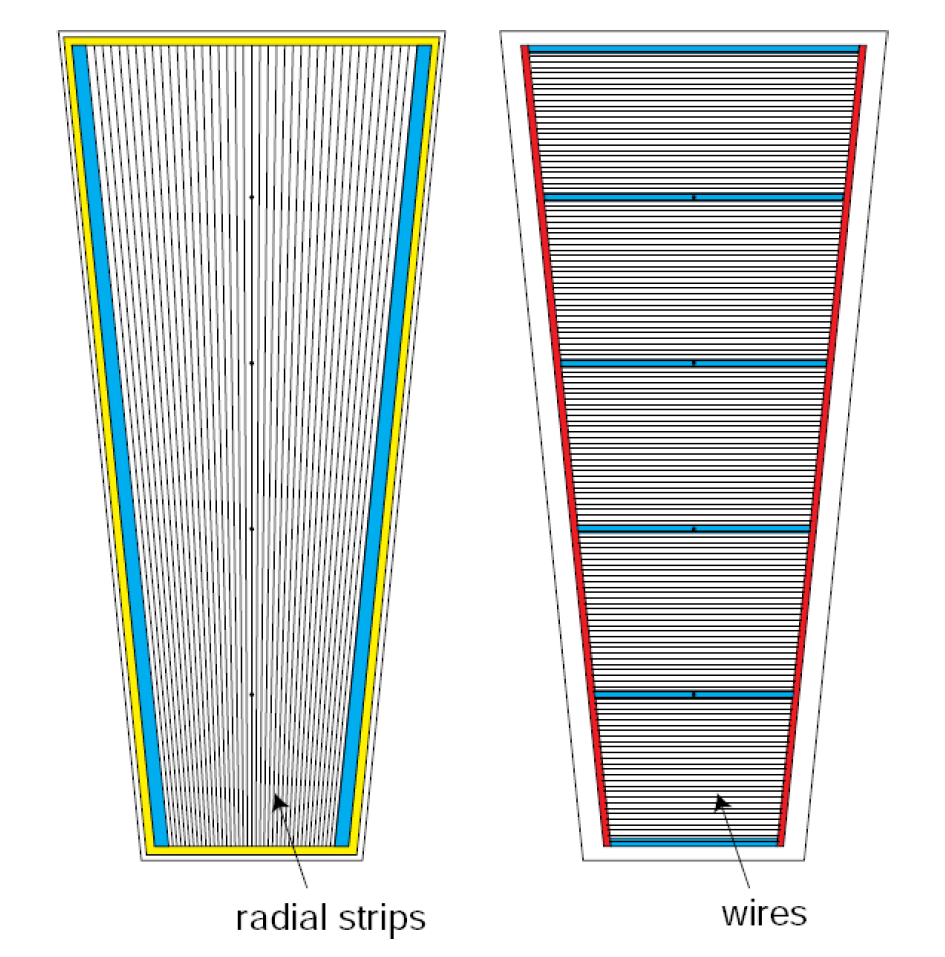
\includegraphics[width=0.5\textwidth]{images/csc.png}
\caption{Schematic representation of CSC cathode (left) and anode (right) panels.}\label{fig:csc}
\end{figure}

RPCs are used both in barrel and endcaps, complementing DT and CSC systems, in order to ensure robustness and redundancy to the muon spectrometer.
RPCs are gaseous detectors characterized by a coarse spatial resolution but able to perform precise time measurements, comparable with the ones provided by scintillators. These chambers are made of 4 bakelite planes, with a bulk resistivity of $10^{10}\mbox{--}10^{11}\,\Omega$cm. The 2\,mm gap between the plates is filled with a mixture of $\mathrm{C_2 H_2 F_4}$ (94.5\%) and Isobutane. 
The central part of the chamber is equipped with insulated aluminum strips, used to collect the signal generated by crossing particles. In the barrel the strips are rectangularly segmented and run along the beam axis, whereas the endcaps are equipped with trapezoidal shaped strips. The detector operates in avalanche mode, and covers the region $|\eta|<2.1$.

